\chapter{Multi-agent software engineering}

\section{Engineering principles}

Specialization can increase coverage by separating implementation, review and verification. It can also amplify cost, correlated mistakes and conflicting edits. The coordinator owns the dependency graph, task allocation and merge order; workers own only their assigned workspace. Shared memory is a coordination channel and potential injection surface, not a source of authority.\src{O6,A5}

\section{Implementation approach}

Represent the task graph as explicit dependencies. Allocate distinct branches and worktrees, assign disjoint file scopes and share immutable task contracts. Implementers produce patches and evidence. A reviewer receives the candidate diff and requirements in a read-only environment. A separate trusted verifier runs checks. The coordinator rejects overlapping changes or creates a new integration task. Cap total workers and aggregate time.

\section{Verification and limitations}

Require each result to identify base and candidate commit; verify integration after merging. If a single agent plus tests achieves the same outcome at lower cost and risk, prefer it. Do not treat agreement between two models as independent proof.

Figure~\ref{fig:d15} illustrates the conceptual flow from Task graph to Integration gate. The edges describe the proposed integration or control relationship, not undocumented internal calls.

\begin{figure}[htbp]\centering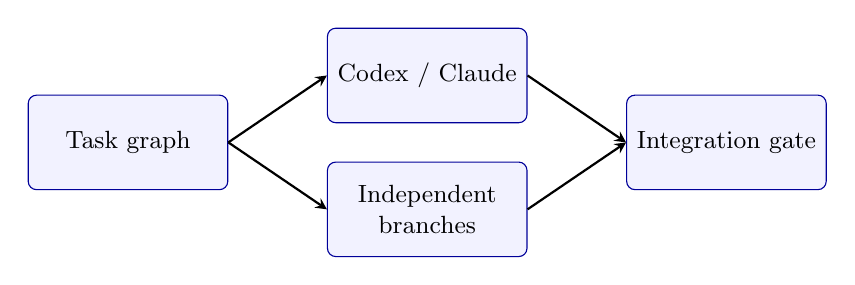
\begin{tikzpicture}[nodebox/.style={draw=blue!60!black,fill=blue!5,rounded corners=3pt,minimum height=12mm,text width=23mm,align=center,font=\small},>=stealth]
\node[nodebox] (n0) at (0.00,0.00) {Task graph};
\node[nodebox] (n1) at (3.80,0.85) {Codex / Claude};
\node[nodebox] (n2) at (3.80,-0.85) {Independent branches};
\node[nodebox] (n3) at (7.60,0.00) {Integration gate};
\draw[->,thick] (n0.east) -- (n1.west);
\draw[->,thick] (n0.east) -- (n2.west);
\draw[->,thick] (n1.east) -- (n3.west);
\draw[->,thick] (n2.east) -- (n3.west);
\end{tikzpicture}
\caption{Multi-agent collaboration (conceptual view).}\label{fig:d15}\end{figure}

\section{Chapter conclusion}

Apply the stated verification criteria before expanding the scope of this workflow. Record deviations, evidence and unresolved risks in the task record.
